
The rocket, entitled RORO I, is a 8 feet (2.45 meters) rocket propelled by a M-class solid motor. The main requirements of the rocket are presented in Table \ref{table:se_topLevelR}.

\begin{table}[h!]
\centering
\begin{tabular}{|p{0.9\columnwidth}|}
\hline
    The rocket shall achieve an apogee of 10,000 ft (3048 meters).  \\ \hline
    The rocket shall have a static margin between 1 and 2 body-calibers \\ \hline
    The rocket shall carry a COTS barometric pressure altimeter with on-board storage as primary data source for altitude reporting.  \\ \hline
    The launch vehicle shall follow a "dual-event" recovery \\ \hline
    The rocket shall carry a minimum mass of 8.8 lb (4 kg) of payload. \\ \hline
    The rocket shall eject its nosecone at apogee. \\ \hline
    The rocket shall release a glider from the payload section at 10 seconds after apogee. \\ \hline

\end{tabular}
\caption{Top Level Requirements for the rocket}
\label{table:se_topLevelR}
\end{table}


\subsection{Design and Manufacturing}


The rocket is divided into 3 main sub-assemblies (Figure \ref{f:rocket_adnoted}:
\begin{enumerate}
    \item The nosecone - carrying avionics and an ejection system
    \item Upper Body - carrying the payload, the parachutes and the recovery electronics
    \item The Lower Body - containing logging avionics and the motor
\end{enumerate}
The concept of the rocket was well-thought to be easy to integrate and robust, considering the time constrains. The rocket separated in the middle, between the upper and lower body. This approach is very common in High Power Rocketry (HPR) and is considered a less risky approach.

\begin{figure}[h!]
\centering
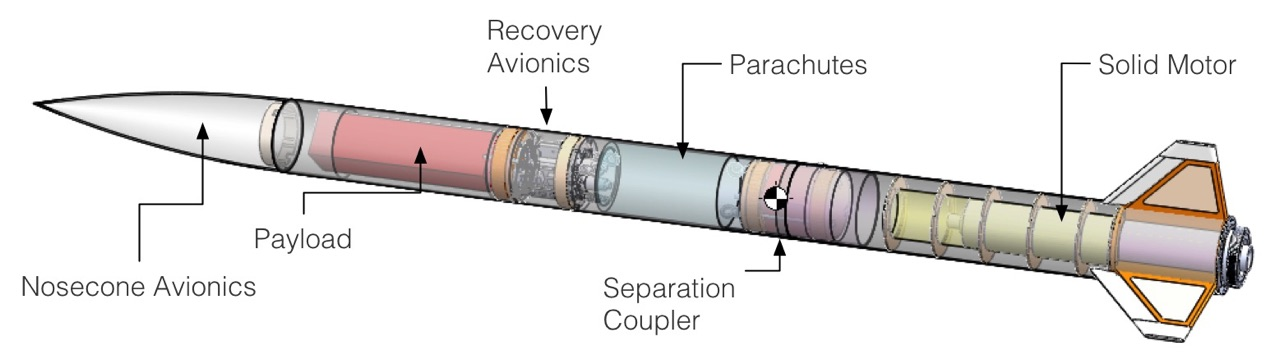
\includegraphics[width=0.5\textwidth]{img/rocket_sw_annotated.jpg}
\caption{The rocket with its main components}
\label{f:rocket_adnoted}
\end{figure}

The length as well as the diameter of the rocket were chosen in such a way to accommodate the payload which had a dimension constraint imposed by the competition (needed to be Cubesat standard).

Two important factors are important in a rocket: the dynamic stability and the static stability.


Now, the manufacturing of each part of the rocket is discussed.



\paragraph{Structure}
\hfill \break
The main body of the rocket is a COTS phenolic tube, reinforced with two layers of 245 g/m$^2$ twill weaved carbon fiber. The reinforcement rational was determined using FEA (Finite Element Analysis), and tested during two rocket flights.
The structure contains also a coupler tube, that is made out of phenolic tube reinforced inside again with two 245 g/m$^2$ layers carbon fiber.
The rocket has two structural bulkheads, one in the lower body and one in the upper body to which the parachute cords are attached. The bulkheads were made out of two 15mm plywood plates reinforced with 4 layers of 245 g/m$^2$ carbon fibre on each side.  The bulkheads are the structurally critical elements as they transfer loads from the rocket body to the subsystems. They need to withstand both the accelerations from the launch and the parachute opening shock. 
The two bulkheads are subject to a peak load of 10kN from the parachute opening shock. An FEM analysis taking into account the  ECSS-E-HB-32-21A revealed that an additional reinforcement of the bulkheads with carbon fibre is required to sustain the loads. The analysis of the bonding to the rocket body reveals sufficient strength to sustain the opening shock.


\paragraph{Fins}
\hfill \break
    The fins were sized for 1.1 calibers static stability %Reference to static/dynamic stability
    The fins were manufactured out of wood and carbon fiber, as it can be seen in Figure \ref{f:fins}. Firstly, the wood was cut at CNC (Figure \ref{f:fins} a). The inside of the fins was made out of balsa wood (Figure \ref{f:fins} b), in order to decrease the weight for higher resonance frequencies. Afterwards, on each side of each fin, 3 layers [span, chord, span] of 140 g/m$^2$ unidirectional carbon fiber were applied, to increase stiffness (Figure \ref{f:fins} c). The fins were attached to the motor tube using high temperature epoxy, reinforced with carbon fiber.
    \begin{figure}[h!]
        \centering
        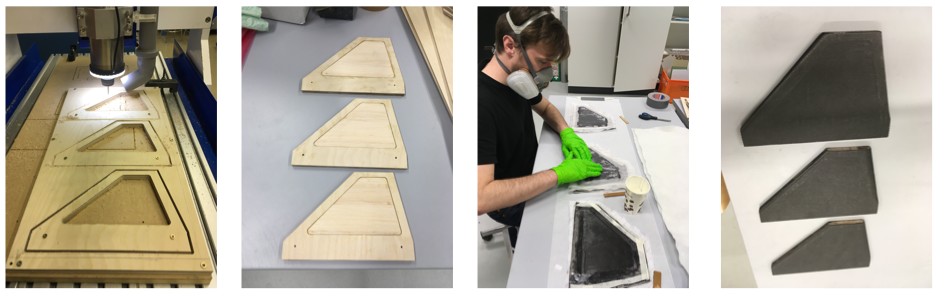
\includegraphics[width=0.5\textwidth]{img/fins.png}
        \caption{a) Wood at CNC b) Final wood-made fins c) Carbon fiber manufacturing d) Final version of the fins.}
        \label{f:fins}
    \end{figure}


\paragraph{Motor tube}
\hfill \break
The motor tube consists of a Commercial-Off-The-Shelf phenolic tube. The fins were glued with 3M DP760 high-temperature epoxy to the motor tube. The tube was centered to the outer rocket body tube by six 4mm plywood centering rings distributed in equally along the motor tube.
In front of the fins, there is a 12mm CNC-cut plywood ring from which 12 M3 threaded rods connect to the thrust plate. These help holding the motor inside the rocket body during parachute opening shock.
The entire assembly can be seen in Figure \ref{f:reinforcement} c. The fins were fixed to the outer structure using ribbons of carbon fiber both on the inside and the outside of the tube, as it can be seen in Figure \ref{f:reinforcement} a,b.

  \begin{figure}[h!]
\centering
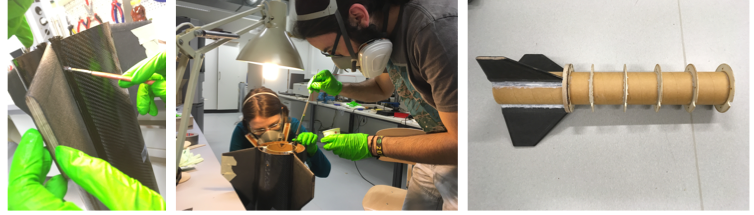
\includegraphics[width=0.5\textwidth]{img/fins_glue.png}
\caption{a, b) Reinforcement of the fins c)Motor tube assembly, with fins and centering rings}
\label{f:reinforcement}
\end{figure}


\paragraph{Motor case}
\hfill \break
The motor case, which is a RMS-98/7680 from Aerotech is held by a 98mm retainer from Aeropack on a custom made laser-cut aluminum thrust plate. The thrust-plate pushes directly on the fins which go through the body tube to the motor tube. The thrust-plate is used to attach the motor and to distribute the loads when parachute opens.
 The retainer \& thrust-plate assembly can be seen in Figure \ref{f:motor_retainer_2}.
\begin{figure}[h!]
        \centering
        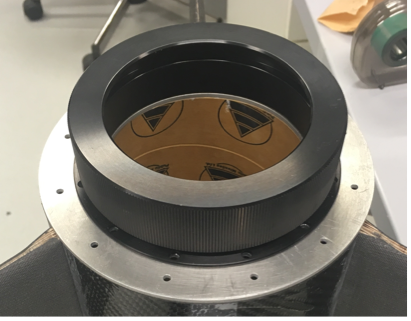
\includegraphics[width=0.3\textwidth]{img/motor_retainer.png}
        \caption{Motor Retainer and the Aluminum plate}
        \label{f:motor_retainer_2}
    \end{figure}


\paragraph{Payload}
\hfill \break
In the lower body of the rocket, there is 1U of payload consisting of 4kg of tungsten and a board with sensors used to track the lower body motion and shocks, referred to as the Logging Electronics. A Gopro and a PCB cameras are also placed to film the parachute deployment and the outside.
The Active Payload bay, placed in the Upper Body, consists of a 4U plywood box reinforced with glass fibre to withstand the loads. Inside the 4U wood box, a glider is mounted on a rail. Shortly after apogee, the glider will be ejected from the rocket using a spring. A more detailed description of the glider will be detailed in the second part of the article.



\subsection{Recovery}

Apart from the aforementioned parts, the rocket's flight is based on a dual-event recovery.

\subsection{Avionics}



\subsection{Flight Tests-PATRICK}